\chapter{Conclusione \workinprogress}

\begin{comment}
Conclusioni

Al momento di scrivere le conclusioni spesso si rimette mano anche all'introduzione poiché sono due sezioni tra loro collegate. Non occorre ripetere quindi le conclusioni già inserite eventualmente nei vari capitoli, ma piuttosto inserire una breve analisi del lavoro svolto, delle problematiche affrontate e delle metodologie per risolverle e indicare possibili futuri sviluppi.

scaletta
    1. sta tesi è una guida implementativa
    2. sta architettura è stata implementata su apparati reali
    3. per la tesi l'architettura è stata simulata
        1. quindi ci stanno delle differenze, es ho usato openwrt stock
    4. evoluzione futura multi-istanza usando una pki perogni processo vpn


\end{comment}

L'architettura proposta in questo elaborato è stata effettivamente implementata su apparati reali durante il tirocinio in collaborazione con l'azienda \it{Esse-ti}. Per rendere più completo il prodotto è necessario modificare la configurazione per consentire che più clienti, ognuno con il proprio Router 4G, possano usufruire del servizio. Si deve però stare attenti a mantenere l'isolamento tra i clienti, per evitare che i dati trasmessi da un cliente vengano letti dagli altri.

A livello implementativo ciò significa avere più di un servizio OpenVPN nel \it{Server}, ogni uno collegato a una \it{Certificate Authority} differente.

Ad esempio con 2 clienti si avrà un'architettura virtuale simile a fig.~\ref{fig:diag2-multiistanza_virtual}, che corrisponde ad una topologia relale in fig.~\ref{fig:diag2-multiistanza_real}.

\begin{figure}[h]
    \centering
    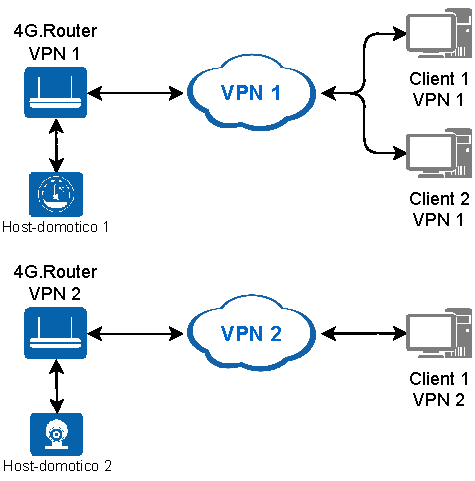
\includegraphics[width=0.6\linewidth]{immagini/diag2-multiistanza_virtual}
    \caption{multi-istanza virtual}
    \label{fig:diag2-multiistanza_virtual}
\end{figure}


\begin{figure}
    \centering
    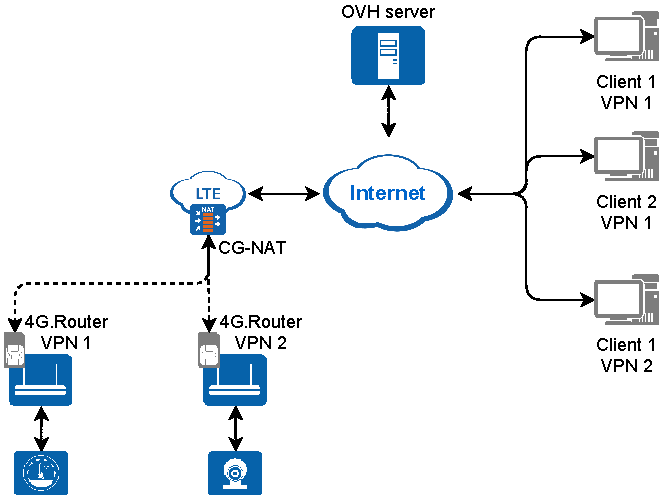
\includegraphics[width=0.8\linewidth]{immagini/diag2-multiistanza_real}
    \caption{multi-istanza real}
    \label{fig:diag2-multiistanza_real}
\end{figure}



